\documentclass[a4paper, 12pt]{article}
% math symbols
\usepackage{amssymb}
\usepackage{amsmath}
\usepackage{mathrsfs}
\usepackage{physsummer}


\usepackage{enumitem}
\usepackage[margin = 2cm]{geometry}

\tolerance = 1000
\emergencystretch = 0.74cm



\pagestyle{empty}
\parindent = 0mm

\begin{document}

\begin{center}
  \Large{\textbf{Городской центр физического образования, 10 класс.}\\
  \textit{Серия 25, 30 апреля 2015.}}
\end{center}

\Large

\begin{center}
  \Large\textbf{ Повторение магнитного поля. }
\end{center}

\task{ По двум параллельным плоскостям текут токи с линейной
  плотностью $j$ в одном направлении. Притягиваются плоскости или
  отталкиваются? Найти силу, действующую на единицу площади
  плоскости. }

\task{ Кольцо радиуса $R$, по которому циркулирует ток $I$, поместили
  в неоднородное аксиально-симметричное поле. Ось кольца совпадает с
  осью симметрии магнитного поля. Индукция магнитного поля $B$,
  действующего на ток, направлена под углом $\alpha$ к оси симметрии
  поля. Масса кольца $m$. Определите ускорение кольца. }

\taskpic{ Прямой провод имеет виток радиуса $R$. По проводу течёт ток
  $I$. Определите индукцию магнитного поля в центре витка и на его оси
  на расстоянии $h$ от его центра. }
{
  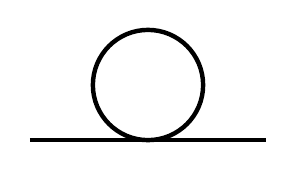
\begin{tikzpicture}
    \draw[ultra thick] (0,0) -- (3,0);
    \draw[ultra thick] (1.5,0.7) circle (0.7cm); 
  \end{tikzpicture}
}

\task{ Металлическое кольцо разорвалось, когда ток в кольце был
  $I_0$. Сделали точно такое же кольцо, но из материала, предел
  прочности которого в десять раз больше. Какой ток разорвёт новое
  кольцо? Какой ток разорвёт новое кольцо, сделанное из этого более
  прочного материала, если все размеры нового кольца в два раза больше
  размеров старого? }

\end{document}


%%% Local Variables: 
%%% mode: latex
%%% TeX-engine:xetex
%%% TeX-PDF-mode: t
%%% End:
